\chapter{Feature Design} \label{sec:introduction}

\section{Online Sketching Interface}

	\subsection{Overview}

		\begin{figure}[t]
		\centering
		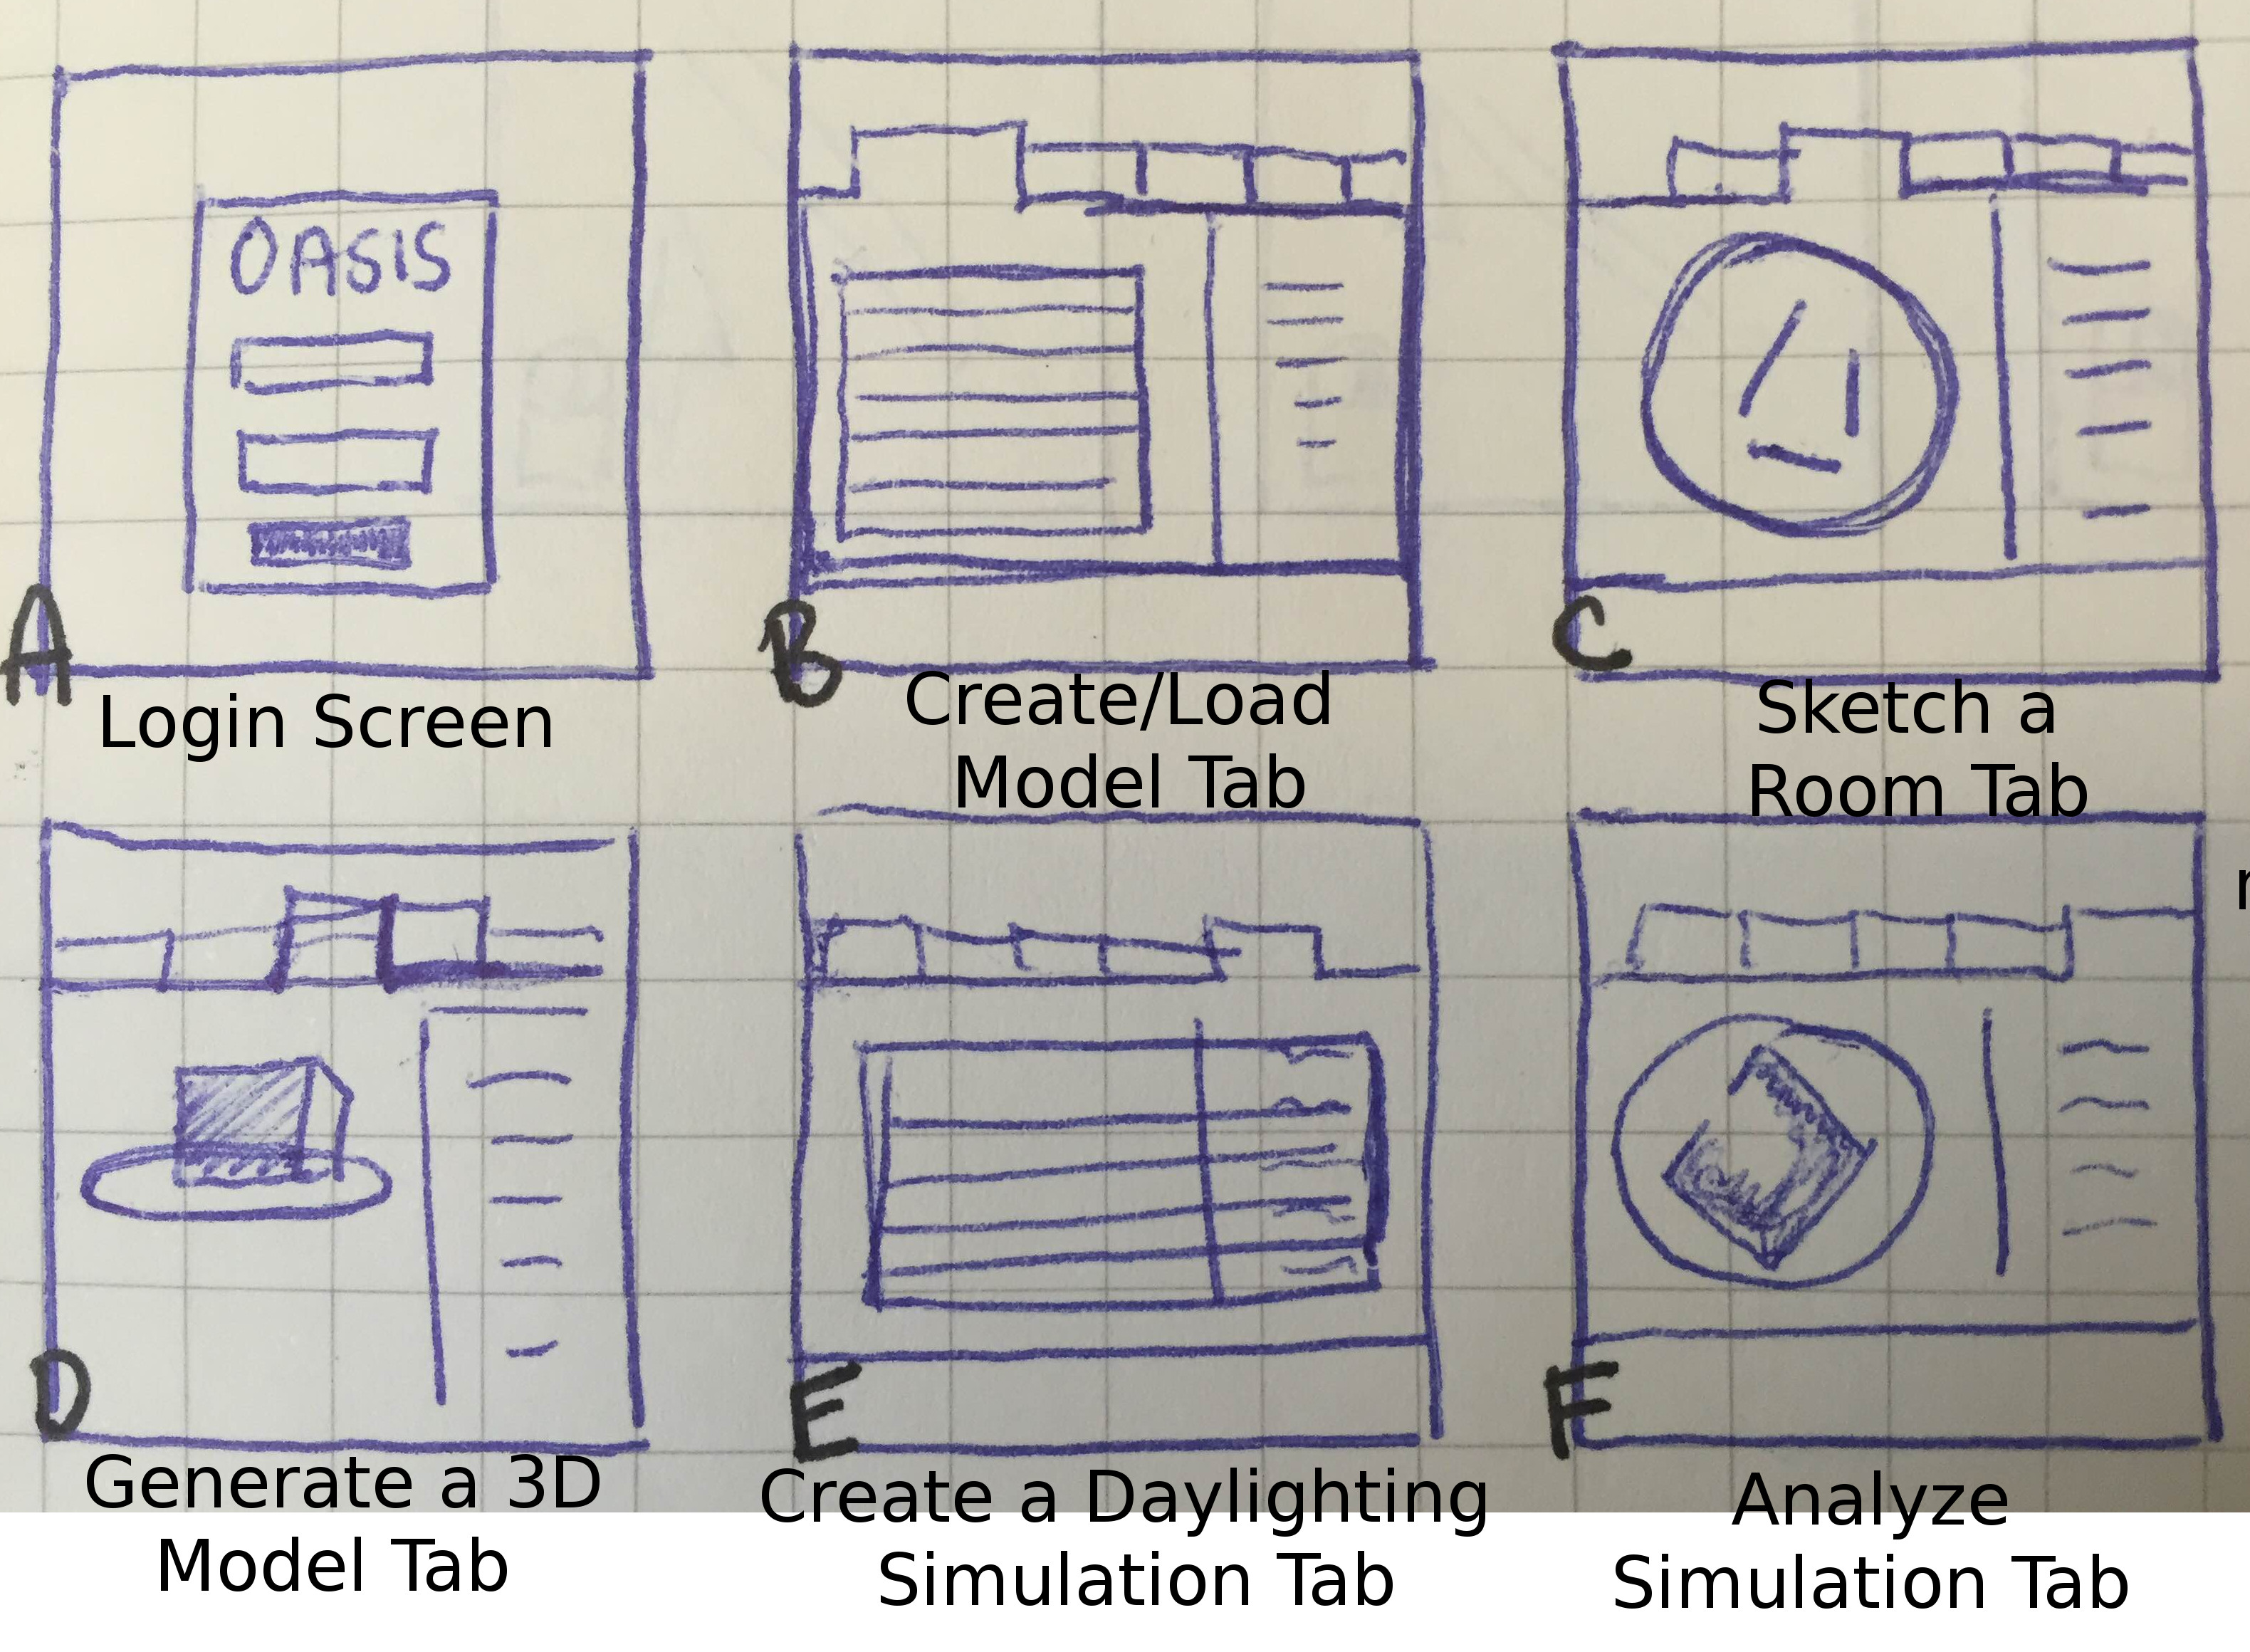
\includegraphics[width=0.8\textwidth]{overview}
		\caption{This is an overview of the tabs and menus available on OASIS. 
		A) login screen 
		B) Create/Load Model tab
		C) Sketch a Room tab
		D) Generate 3D model tab
		E) Create Daylighting Simulation tab
		F) Analyze Simulation Tab}
		\label{fig:overview}
		\end{figure}

		The novel online sketching interface used in OASIS host a variety of features.
		The sketching interface, as seen in figure-\ref{fig:overview} was designed to both familiar and intuitive.
		I used RibbonJS, a JavaScript port of Microsoft's Ribbon user interface, in order to present tools to users in a familiar style\cite{ribbonjs}. 
		The whole interface is broken down into five tabs, as shown in figure-\ref{fig:overview}.
		Each tab has a unique purposes and as a result each tab comes with its own set of buttons.
		Navigation between tabs can be both linear and non-linear. I recommend that beginning users follow tabs linearly. 
		The first tab, known as the \textit{Create/Load Model} tab contains a list of previously made sketches for loading.
		Users can either click on the name of a previously created model or create a new models from the \textit{create/load model} tab.\\

		\begin{figure}[t]
		\centering
		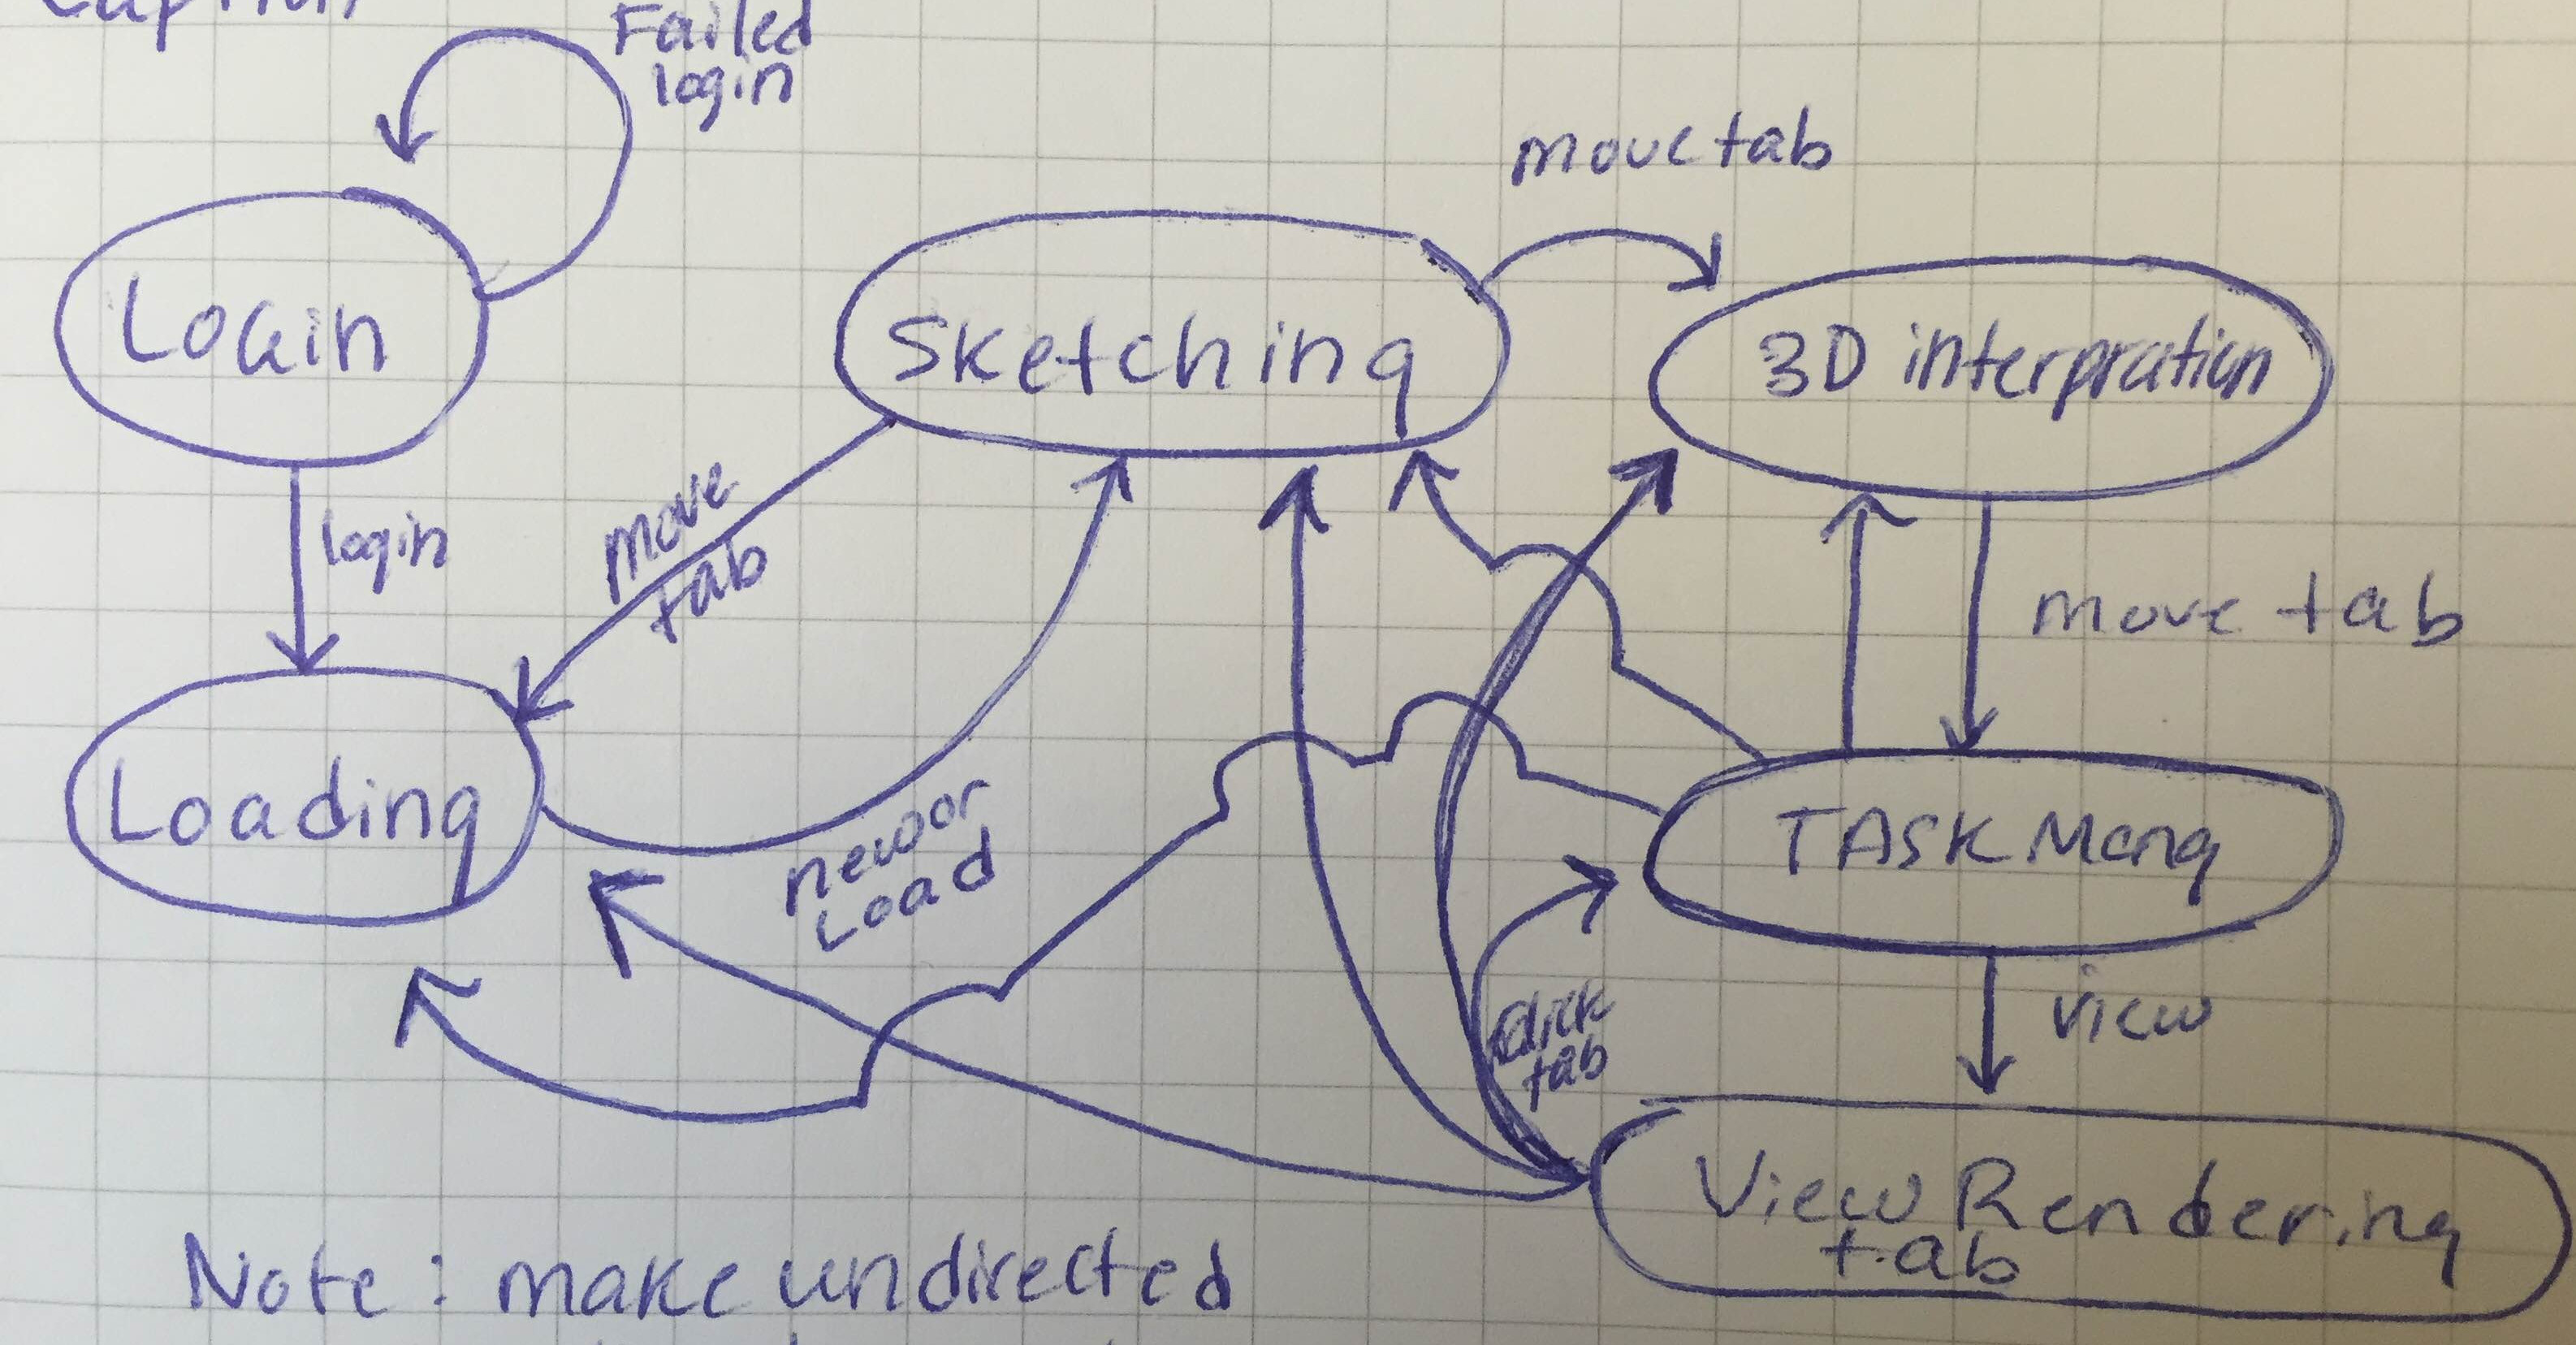
\includegraphics[width=0.8\textwidth]{states}
		\caption{State diagram between tabs and menus on OASIS.}
		\label{fig:states}
		\end{figure}


		Given users follow OASIS linearly, the next tab users navigate to it the \textit{Sketch a Room} tab. In the \textit{Sketch a Room} tab users can design both rooms and floor plans to define architectural spaces.
		After a user has created a sketch, the next tab users navigate to is the \textit{Generate 3D Model} tab. 
		Here users will view a 3D interpretation, without daylighting, of their sketch. 
		Users can then generate daylight renderings by navigating to the \textit{Create Daylighting Simulation} tab.
		While on the \textit{Create Daylighting Simulation} tab users can create new renderings or view previously created renderings.
		Figure-\ref{fig:states} illustrates how tab navigation can be used both linearly and non-linearly in OASIS.
		All in all, we follow familiar user interface visuals and behavior to reduce the learning curve of using our tool and allow users to quickly run daylighting analysis in the fewest number of click possible.\\


		Another framework used in our sketching interface is RaphaelJS\cite{}.
		Raphael JS is a 3D vector graphics library for JavaScript. 
		I use RaphaelJS to handle the 2D graphics created by and objects placed into sketches. I also use RaphaelJS because it supports vectorized lines and objects, allowing our interface  to be re-sizable with lost of visual quality.
		I also use Raphael FreeTransform in conjunction with RaphaelJS\cite{}. 
		The FreeTransform extension is used to create handles on furniture items so that users may easily rotate and reposition these items where they please.
		Figure-\ref{fig:oldvh} demonstrates the handles FreeTransform generates for object manipulation.\\

	\subsection{Usability Features}

		\begin{figure}[t]
		\centering
		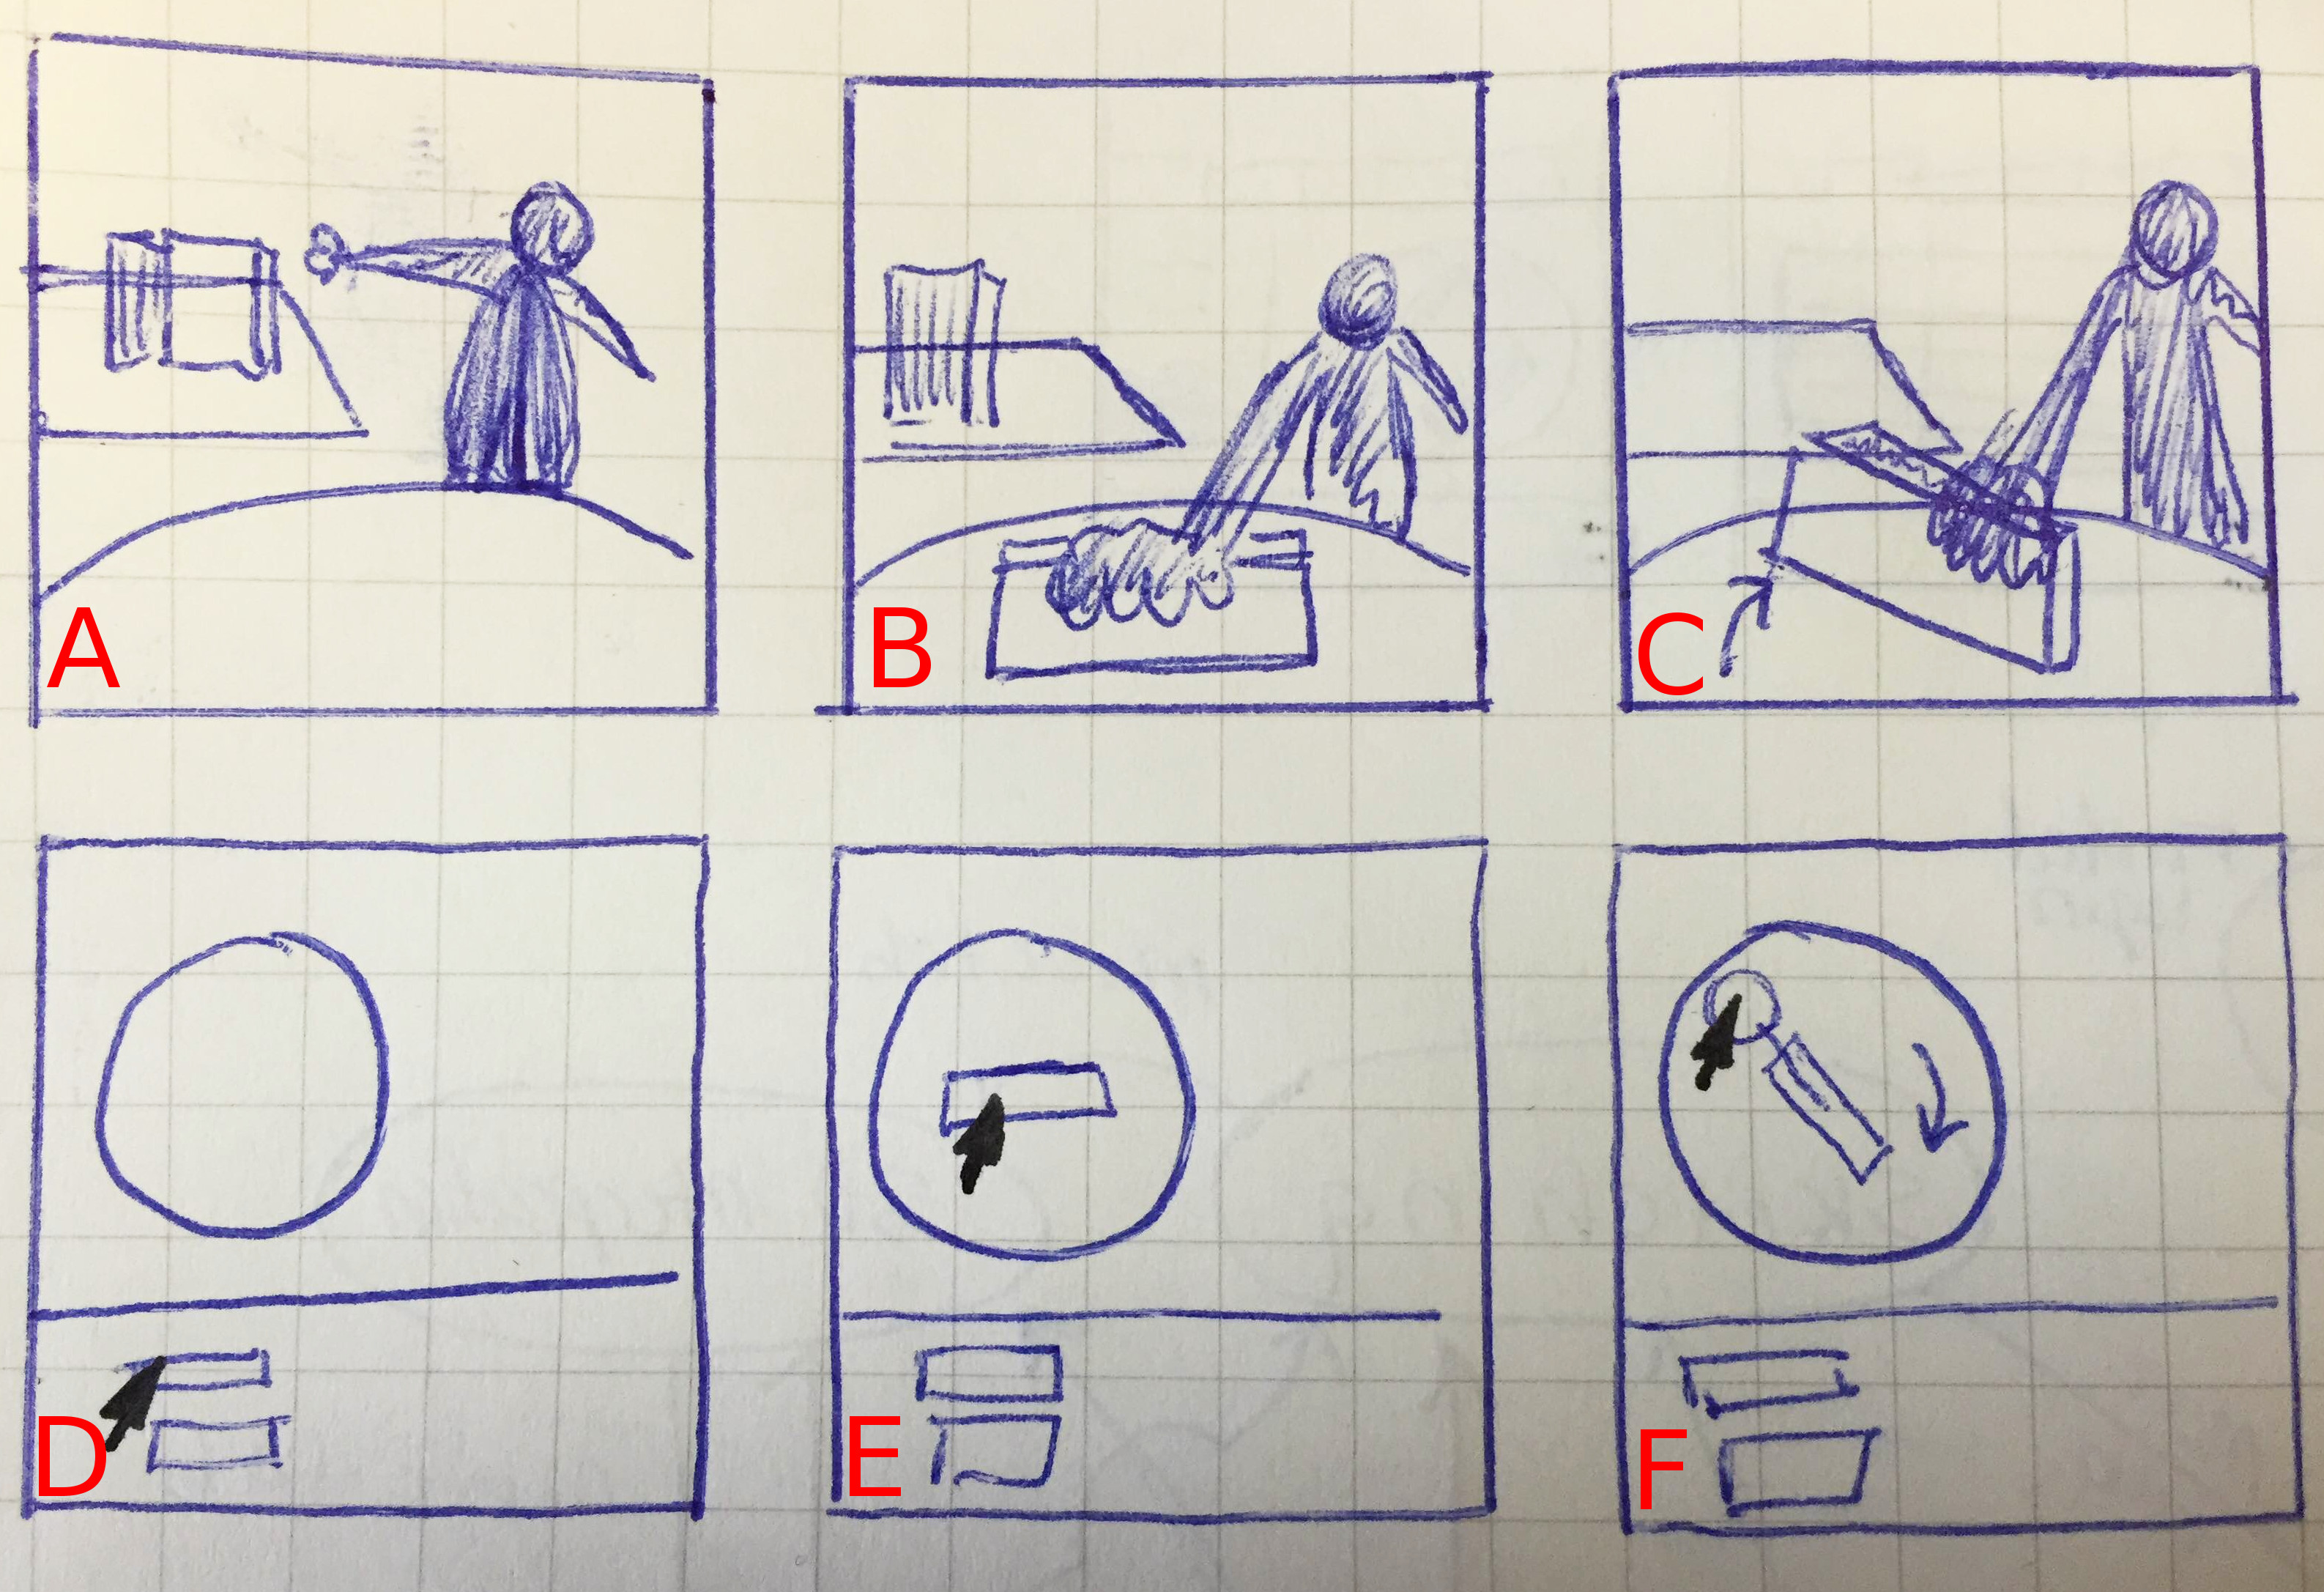
\includegraphics[width=0.8\textwidth]{oldvh}
		\caption{Similarities between old drag and drop interface and the Virtual Heliodon's Tangible User Interface. A) Users select a physical primitive from a collection of primitives. B) Users place primitive on the table top. C) Users adjust the primitive as desired. D) Users select a primitive from a tray on the bottom of the interface. E) Users drag that item onto the table. F) Users use FreeTransform handles to scale and rotate the primitive as desired.}
		\label{fig:oldvh}
		\end{figure}

		There are direct and indirect usability features in the online sketching interface.
		To begin, in order to make the interface as simple as possible I brainstormed the several ways users can place wall and windows onto our sketching interface.
		At first, users could create walls and windows by drag and dropping them into the canvas as showing in figure-\ref{fig:oldvh}.
		Users could then further manipulate walls and windows by both rotating the item around its center axis and by scaling the item though use the FreeTransform handles. 
		Early feedback showed that this approach was both unintuitive and did not translate well into our online sketching interface, despite mimicking how wall primitives were placed in the Virtual Heliodon.
		Figure-\ref{fig:oldvh} shows how users placed walls into a scene on both the virtual Heliodon and on the first version of the online sketching interface.
		My next approach mimics how users draw on paper and in sketching software.
		Users first click on the wall button located in the ribbon of the \textit{Sketch a Room} tab.
		The by clicking and dragging anywhere on the canvas users are shown a preview of where walls will be drawn.
		By releasing the mouse a preview will be replaced by a a drawn line, representing a wall.
		Once a wall is drawn further editing is not allowed, however, users can remove any wall later on.
		To keep with the spirit of sketching, windows are also placed into a sketch by being drawn similarly to walls.
		However, unlike walls, windows need to be on or associated with a wall.
		As a result windows need to be drawn on or near a wall.
		In the interest of the user, windows do not need to be drawn exactly on walls.
		Windows when drawn near walls with similar angles will automatically target snap onto a wall.
		This snapping feature makes drawing windows less relent on users' precision with a cursor, and instead focuses on users' intention.
		Figure-\ref{fig:wall_win} demonstrates how walls and windows are drawn onto the canvas in our sketching interface.

		\begin{figure}[t]
		\centering
		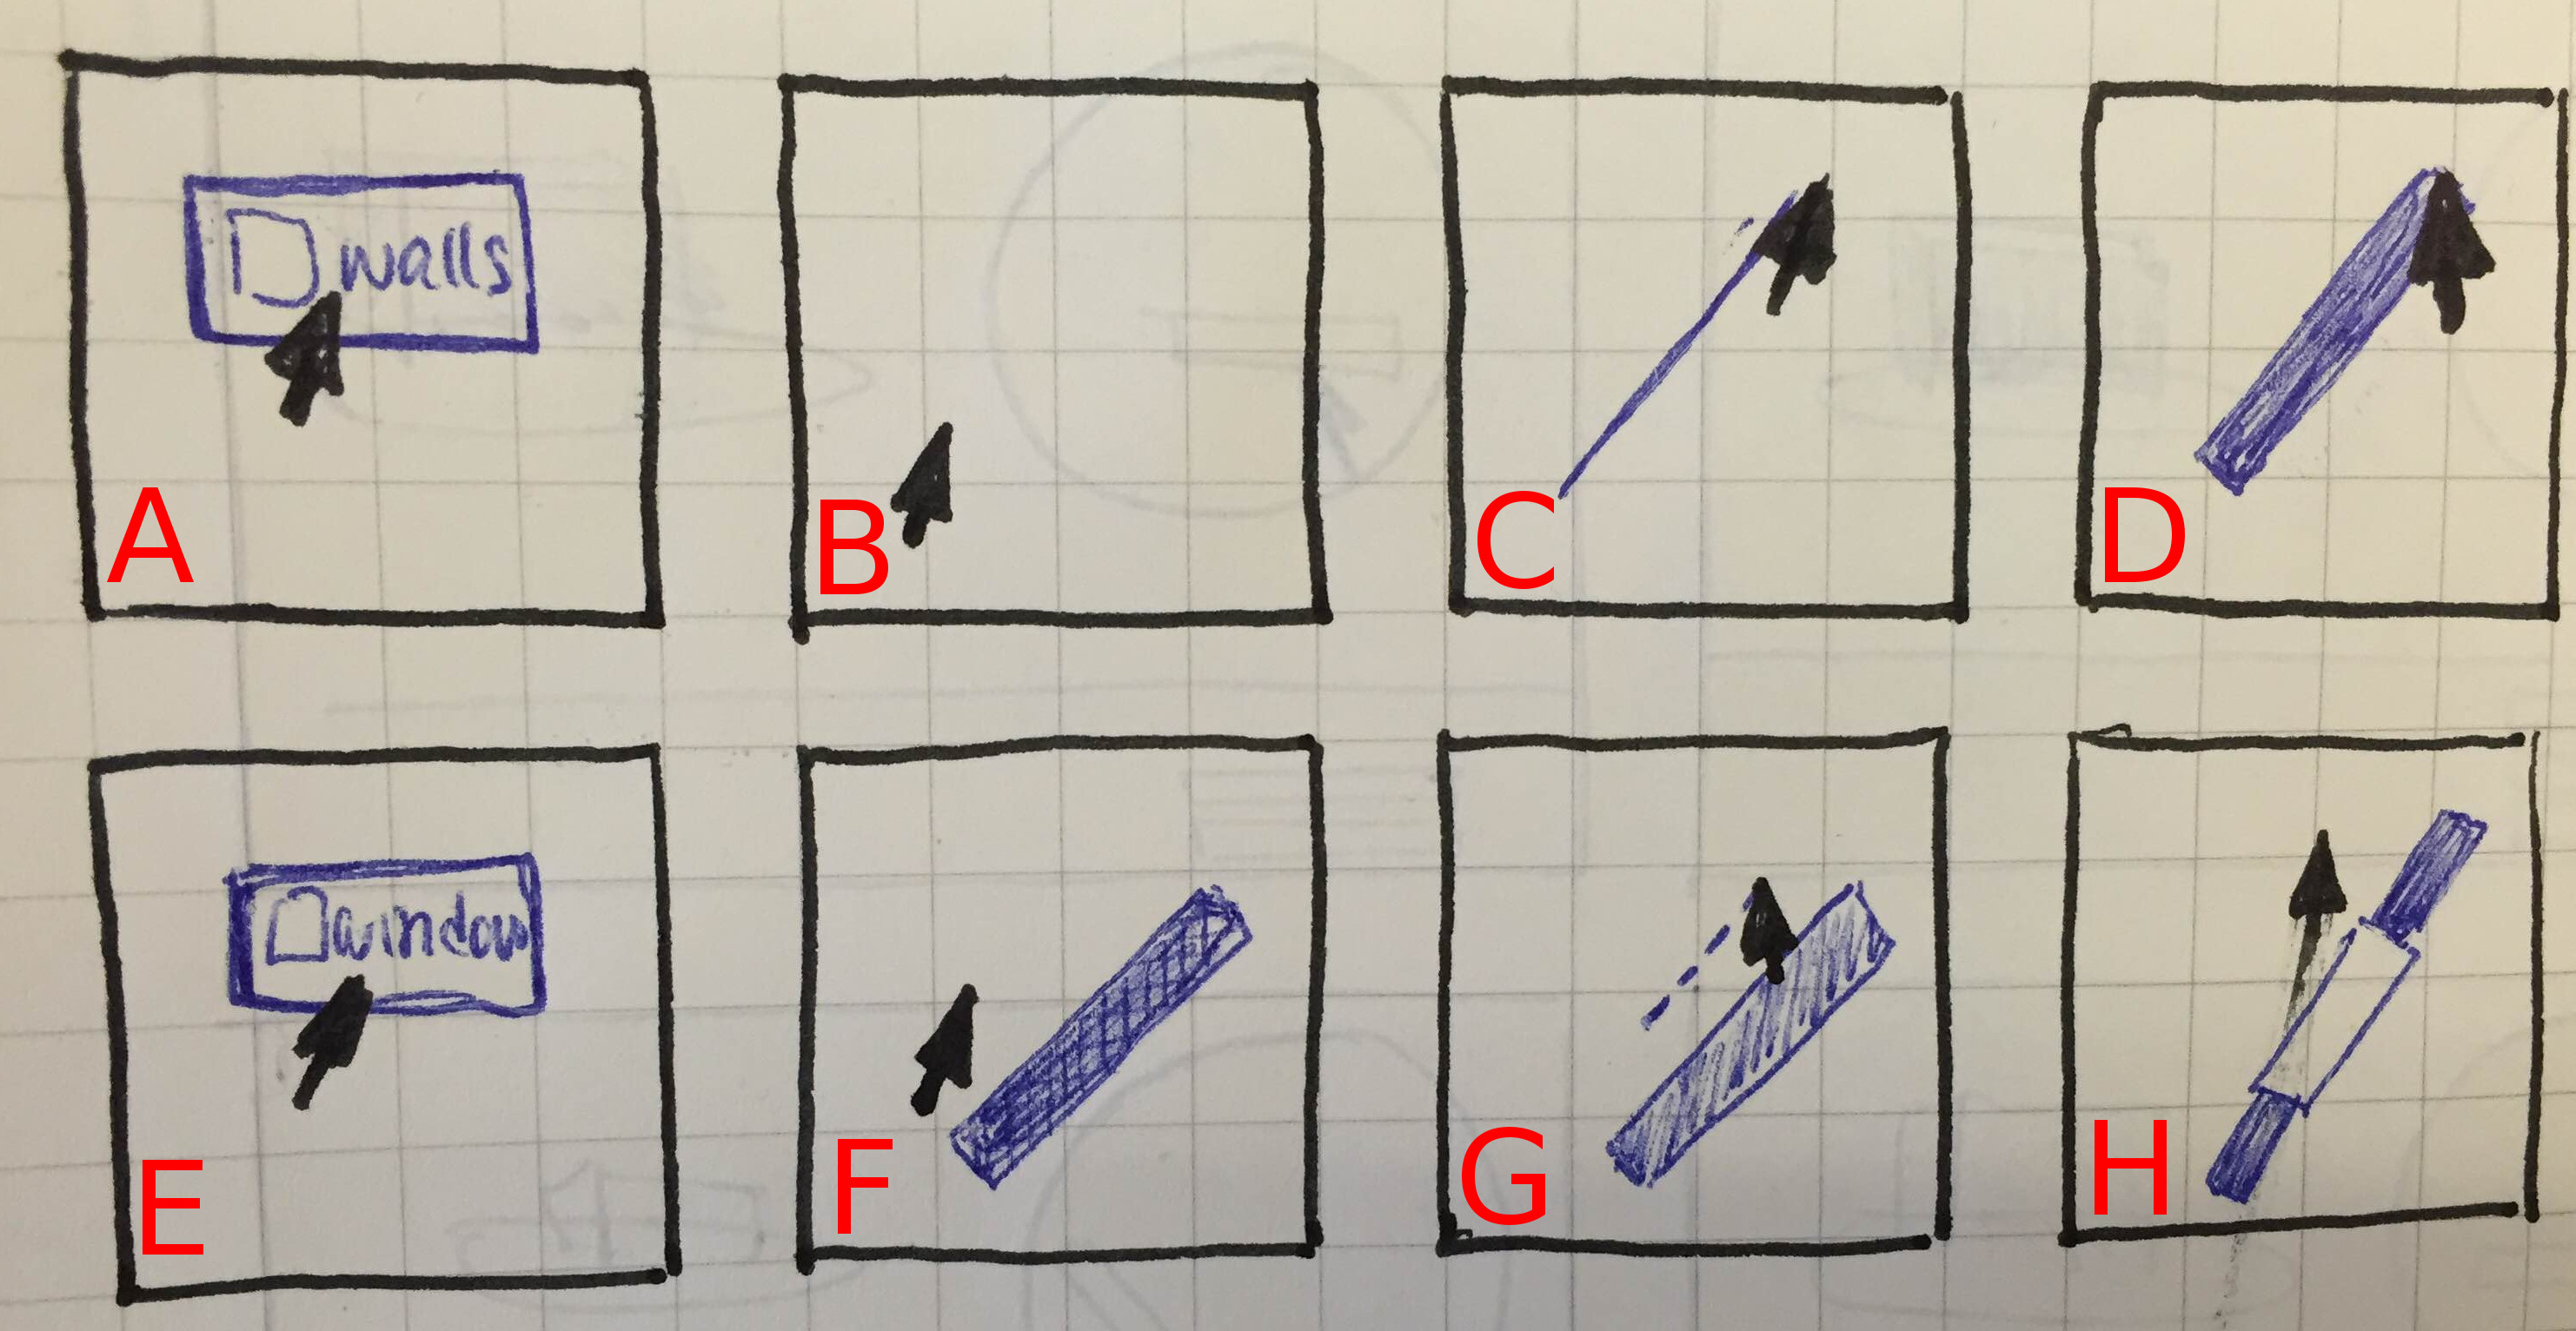
\includegraphics[width=0.8\textwidth]{wall_win}
		\caption{How to create walls and windows on the new sketching interface. A) Users select the wall button located on the ribbon. B) Users click and hold left mouse button anywhere on the canvas. C) Users drag their mouse to desired position while still holding the left mouse button. D) Once define wall location, angle, and length users can release the mouse button and a wall is drawn onto the canvas. E) To draw  windows users first select the window button located on the ribbon. G-H) Users draw windows just as they draw walls, windows will automatically snap to nearby wall upon left mouse button release. }
		\label{fig:wall_win}
		\end{figure}

		Unlike walls and windows, furniture items are placed into the canvas by first clicking on a furniture button  and then manipulating the newly create furniture item via translations and rotations. 
		Furniture items can be rotated along its center axis via FreeTransform handles attached to the furniture item.
		Furniture items can also be translated by clicking and dragging on the item itself.
		The manipulations of furniture items is similar to the manipulation of walls in the original interface as show in Figure-\ref{fig:oldvh}.
		Item manipulations via handles and drag and drop mechanics is a common UI mechanism. 
		Users will be familiar with this mechanism if they have had experience using photo editing software or slide-based presentation tools such as Microsoft PowerPoint\cite{}.
		The removal of all sketch based elements and furniture is simple as well.
		Users must first click on the remove button then click on any items they wish to remove. 
		Walls, windows, and furniture under the cursor will be highlighted red and only removed upon a mouse click.
		Figure-\ref{fig:remove} shows how to remove items on OASIS.

		\begin{figure}[t]
		\centering
		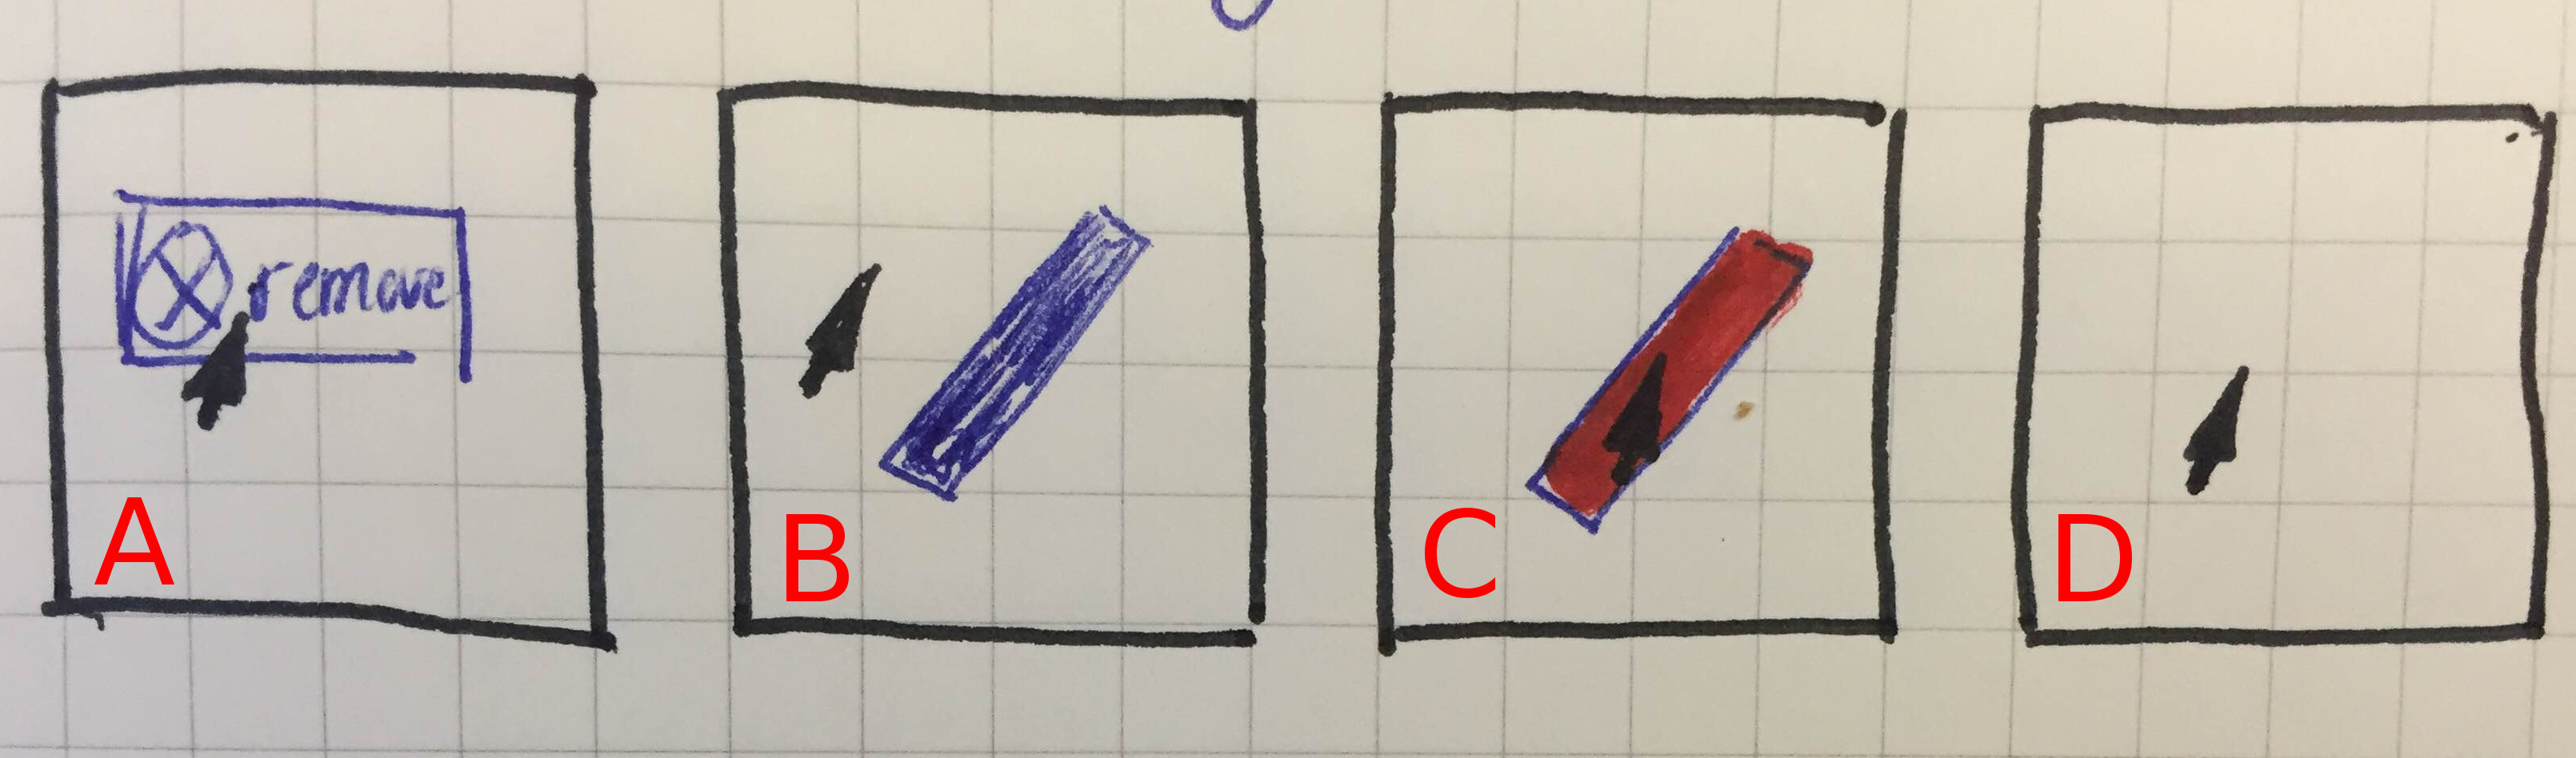
\includegraphics[width=0.8\textwidth]{remove}
		\caption{How to remove an item from the canvas. A) First users must select the remove button located on the ribbon. B) Second the user must move mouse over the time to be deleted. C) Item to be deleted upon left mouse click is highlighted red. D) If the red highlighted item is the correct item to be removed click the left mouse button. }
		\label{fig:remove}
		\end{figure}

		Daylighting varies by many factors.
		Notably, the cardinal orientation of user sketches needs to be defined in order to simulate direct lighting.
		In order to define cardinal orientation on OASIS, users must first click on the orientation button located in the ribbon of the \textit{Sketch a Room} tab.
		Then users can click and drag anywhere on the canvas.
		Holding the left mouse button on canvas will move the North and South labels around the circumference of the canvas to define where North and South are oriented.
		Moreover, daylight varies by geographical location as wall as cardinal orientation.
		To define a geographical location we have users click on the location button located right next to the orientation button.
		Clicking the location button will bring up a map projection where users can select their model's geographical location by clicking anywhere on the map.
		Users do not need to fill in exact latitude and longitude values because we intend OASIS to be an early design tool. 
		Moreover, daylighting varies significantly depending on what hemisphere a model is located. Daylighting also varies depending on a model's location relative to the equator.
		Inaccurately selecting a geographical position off by an entire state or even country will not vary daylighting much.
		Figure-\ref{fig:geoloc} illustrates how a sketch's cardinal orientation and geographical location are defined.

		\begin{figure}[t]
		\centering
		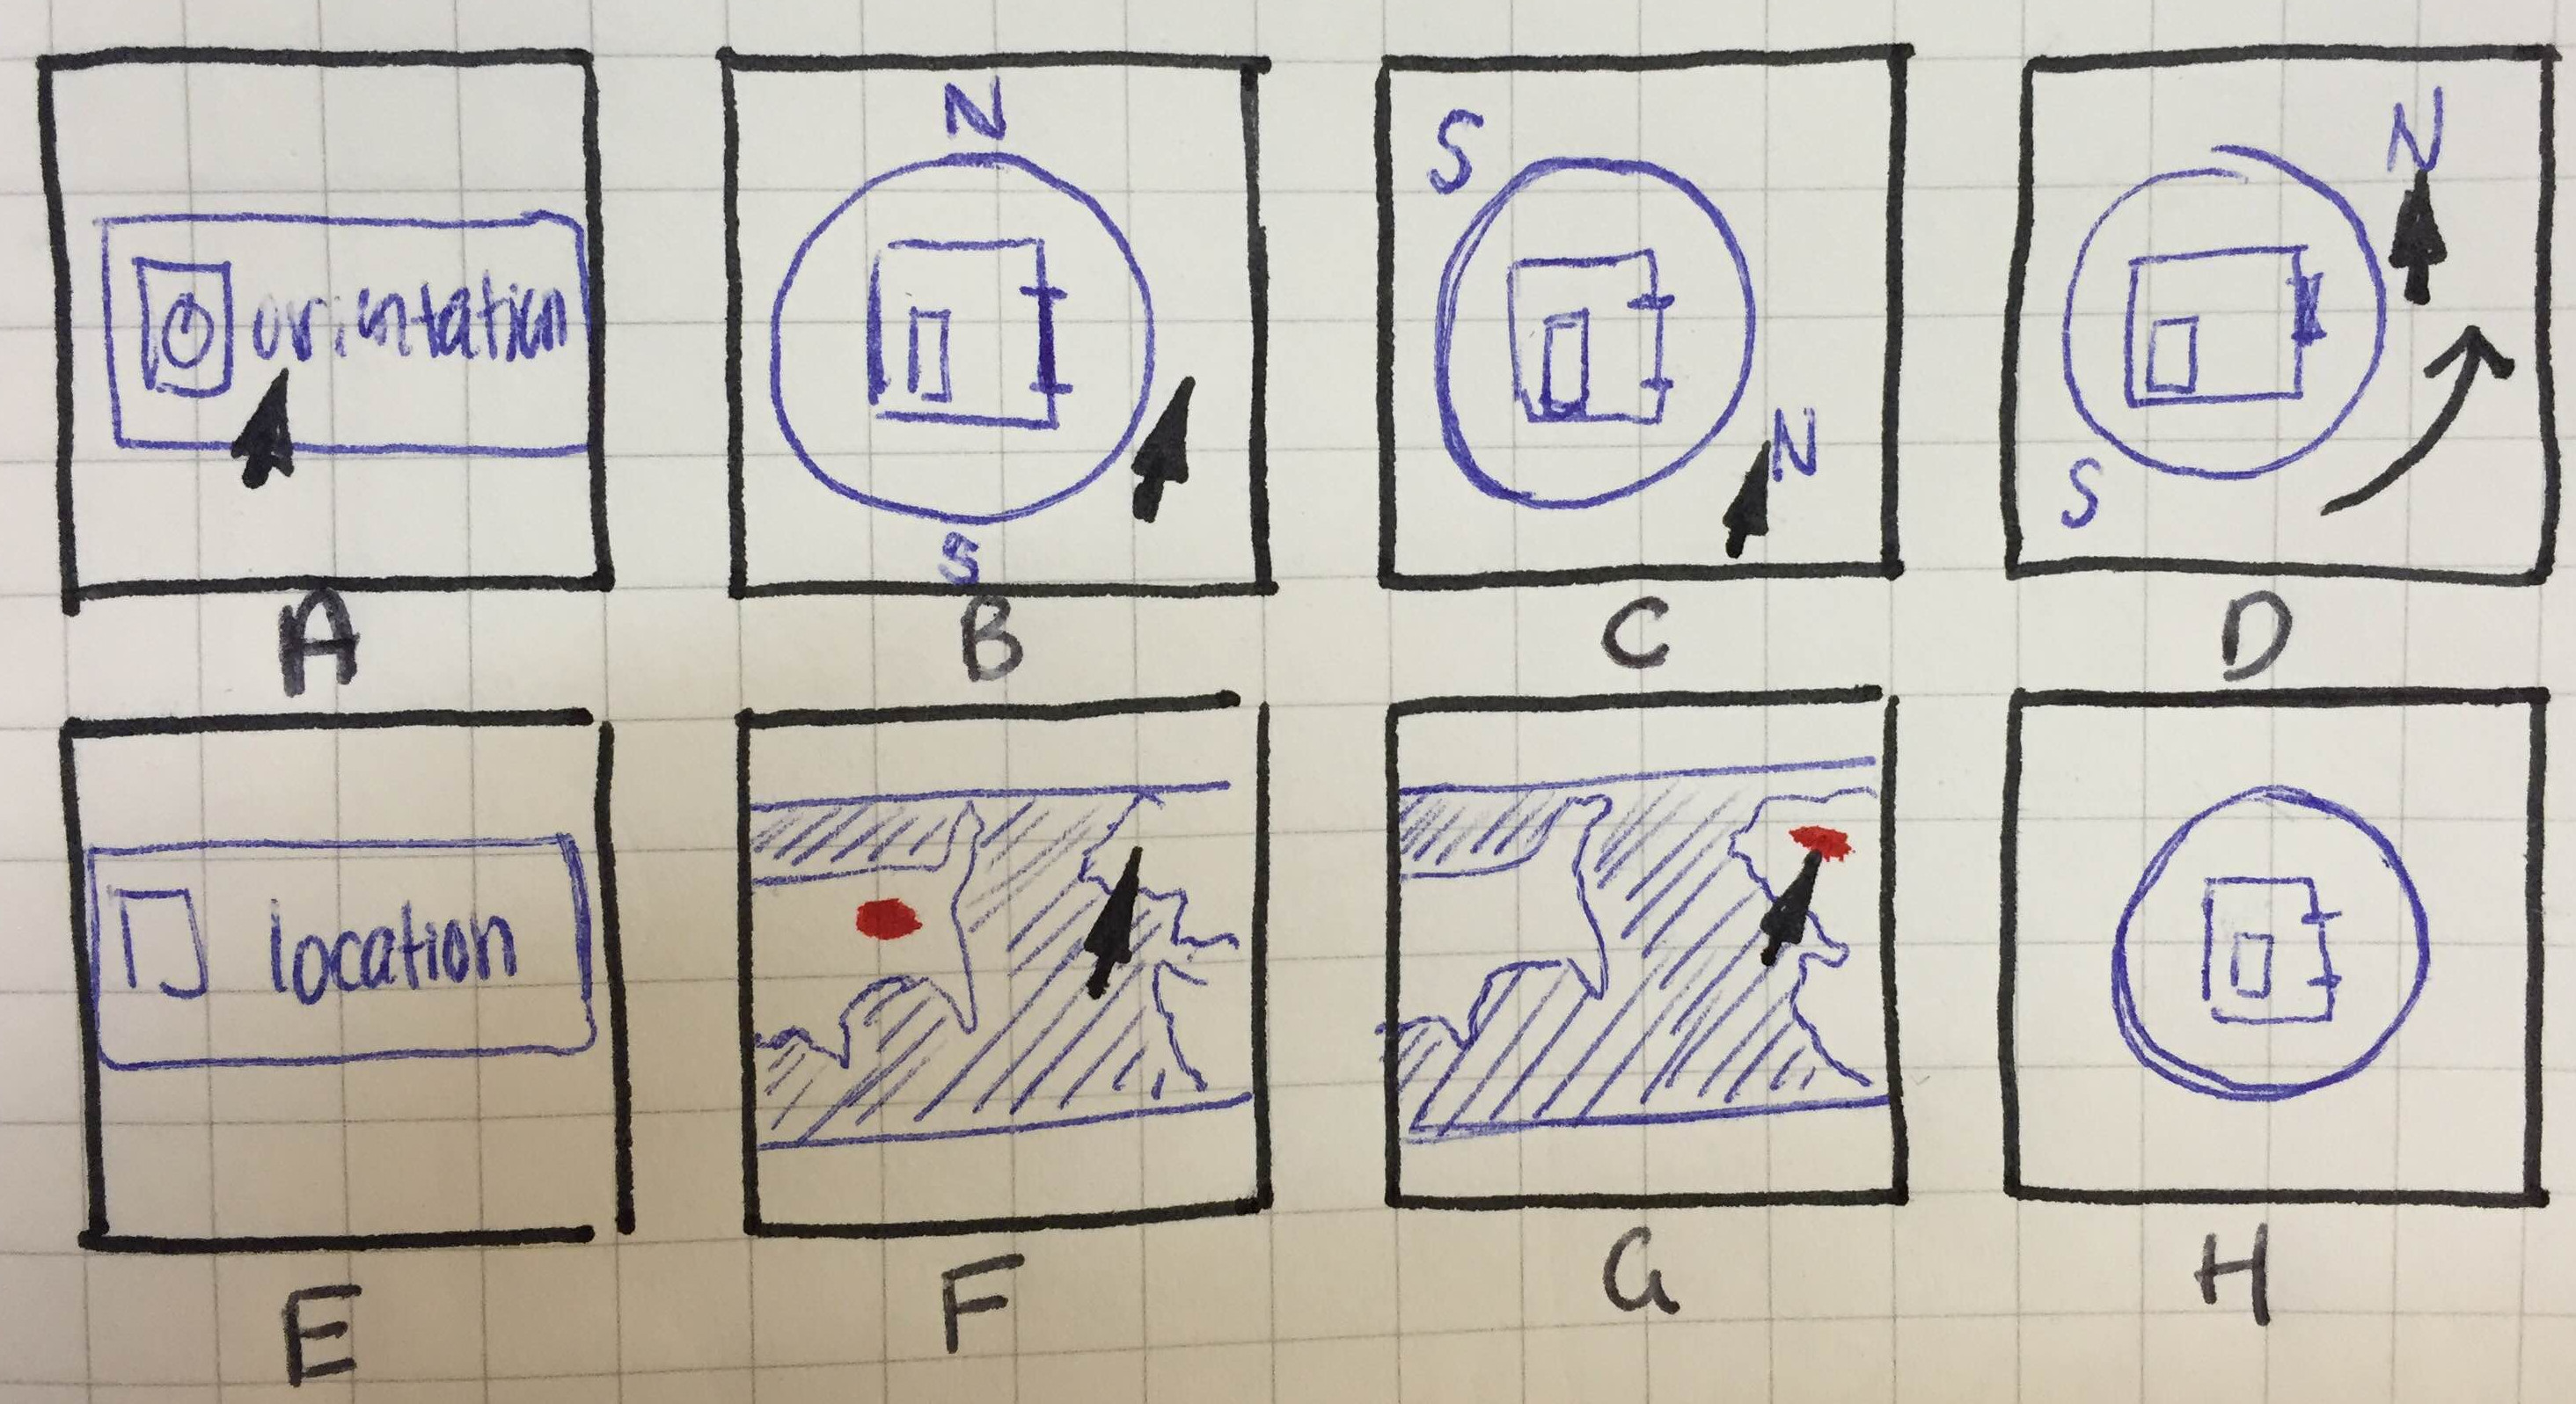
\includegraphics[width=0.8\textwidth]{geoloc}
		\caption{How to set the cardinal orientation and geographical location of a sketch.
		A) To set the cardinal orientation of a sketch first click on the orientation button located in the ribbon.
		B) Press and hold the left mouse button anywhere on the canvas.
		C) Using the North and South labels to indicate cardinal direction continue holding left mouse and move the label to represent desired orientation.
		D) Release the left mouse button and your orientation is set.
		E) To set a geographical location select the location button located in the ribbon.
		F) A map will appear with a default location pinned by a red marker.
		E) Left mouse click the location of the sketch on the displayed map. The marker will move  the new set location.
		F) The map will disappear shortly after setting the new location.}
		\label{fig:geoloc}
		\end{figure}

		Other, not so immediately obvious, usability features supported include an implied sense of scale.
		Adding furniture items of fixed size to the interface implies a sense of scale.
		Statically sized furniture items give users an idea of how big or small other element in a room are.
		Although daylighting is scale invariant, enforcing scale gives us, the researcher, the ability to compare real world spaces with space reproduced in our interface.
		Likewise, to make comparisons between user sketches and 3D models generated by the physical interpretation algorithm easier, I make sure the top down view both models match.
		Lastly, I make sure to automatically save models when users switch between tabs.
		Rather than manually having users save models, we decided that automatically saving models would be one less concern to the user.


\section{3D Model Viewer}

	\begin{figure}[t]
	\centering
	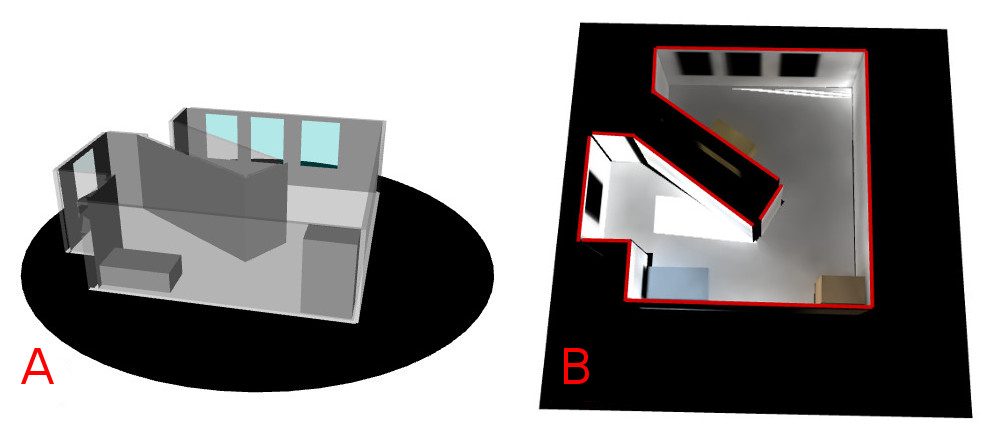
\includegraphics[width=0.8\textwidth]{viewer}
	\caption{ A) Navigable daylight rendering and b) 3D interpreted geometry. There are the two kinds of models we can view in our 3D Model Viewer.}
	\label{fig:viewer}
	\end{figure}

	I use RaphaelJS to manage the 2D elements in OASIS's sketching interface, however we use WebGL to view renderings and 3D interpreted models. 
	Specifically, I use the WebGL library ThreeJS\cite{}.
	ThreeJS is a framework that provides useful wrappers for common WebGL functions.
	WebGL is supported on most web browsers including Google Chrome and Mozilla Firefox\cite{}.
	WebGL gives us the ability to have this sketching interface online in a platform independent manner.
	Our viewer can be used to view both 3D models produced by the physical sketch interpretation algorithm and rendering produced by the daylighting rendering engine as shown in figure-\ref{fig:viewer}.
	The output from both of these components are different and as a result our viewer must be able to handle both texture and non-textured models.
	Output produced by both the physical sketch interpretation algorithm and the daylighting rendering engine is saved as a 3D triangle mesh in a non-standard OBJ file format.
	The OBJ file is the parsed and rendered for viewing with ThreeJS and WebGL.
	Additional, output from the daylighting rendering engine requires the extra step of texture mapping.
	Our viewer lets users change their view of the 3D model though rotation, panning and zooming. Users can press, hold, and drag  the left mouse button to rotate a model along it center axis.
	To zoom in users must hold a modifier key, such as the shift or ctrl key, and press hold and drag their left mouse to zoom in or out.
	Lastly, users can pan a model using the keyboard arrow keys.

	\begin{figure}[t]
	\centering
	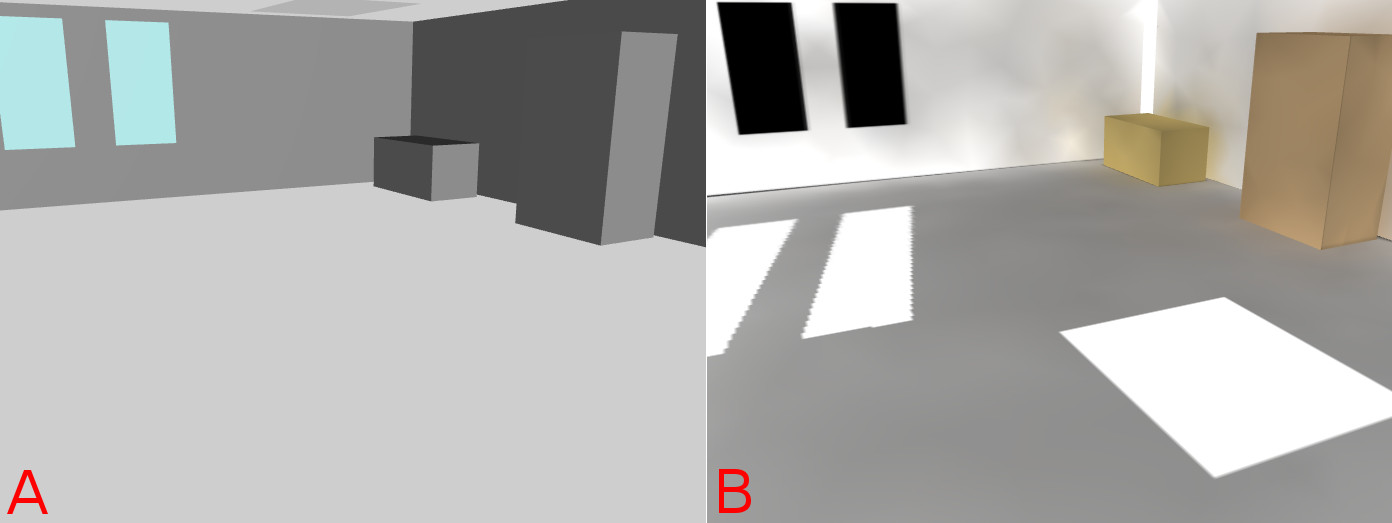
\includegraphics[width=0.8\textwidth]{fps}
	\caption{A and B are examples of zooming into a model to observe a first person point of view.}
	\label{fig:fps}
	\end{figure}

	Aside from basic navigation, there are a couple of usability features build into the viewer.
	Firstly, just as with the sketching interface the viewer can be scaled to fit any web browser window without loss of quality. 
	Also when viewing output from the physical sketch interpretation algorithm, we render walls facing user's viewpoint as transparent, as showed in Figure-\cite{}. 
	These transparent walls  allow users to get a better view models from multiple viewpoints other than the fault overhead view.
	By default the ceiling is not displayed so users can peer into a 3D model from a top down view.
	Furthermore, when viewing output from the physical sketch interpretation algorithm, users can toggle the ceiling as viewable. 
	This is useful if users want to see what portions of the model are interpreted as interior and exterior. 
	The ceiling is useful to see where skylights are located in a model.
	Toggling the ceiling is also useful when zooming into the model to visualize a space from first person point of view -- as shown in Figure-\ref{fig:fps}.
	Additionally, when viewing daylighting renderings, users can toggle between a regular render and a rendering with false color visualizations for locating portions of a room that suffer from over and under illumination.
	Previous work on over and under illumination visualizations by Nasman et al. is used to render blue checkerboard textures on locations suffering of under illumination and re check board textures on locations suffering from over illumination\cite{nasman2013physical}.
	Figure-\ref{fig:false_color} demonstrates how to toggle between false color rendering and normal daylight renderings.
	In short, the 3D model viewer gives users basic navigation functionality, in addition to a handful of other useful features.

	\begin{figure}[t]
	\centering
	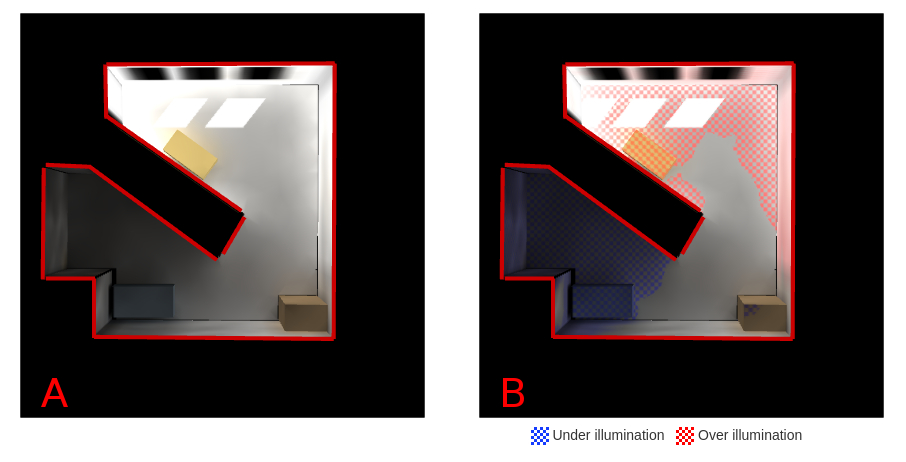
\includegraphics[width=0.8\textwidth]{false_color}
	\caption{An example of false color renderings. A) Is a model that suffers from under illumination in the left most portion. B) Is the same model with false color visualizations toggled. Blue checker-board patterns are used to denote under illumination and red checker-board batter are used to note over illumination.}
	\label{fig:false_color}
	\end{figure}


